\section{Results}\label{sec:results}

\begin{table}[h]
\centering
\small % Adjust font size
\centering
\caption{Scanning performance of TRODO compared with other methods, in terms of Accuracy on standard trained evaluation sets (ACC \%) and adversarially trained ones (ACC* \%). The best results are emphasized in \textbf{bold} format respectively in each column.}
\label{table:main}
% Performance evaluation of our model against various advanced adversarial attacks, measured by ACC (\%), with $\epsilon=\frac{4}{255}$ for low-resolution images and $\epsilon=\frac{2}{255}$ for high-resolution images, Measured by ACC (\%). The best results are emphasized in bold format respectively in each row. The table cells denote results in the "PGD/\graytext{Clean}" format.

\renewcommand{\arraystretch}{1}\setlength{\tabcolsep}{1pt} \Large % Adjust row height
% \resizebox{0.6\linewidth}{!}{\begin{tabular}{lcccccc}
    \resizebox{1\linewidth}{!}{\begin{tabular}{cc*{12}{C{2cm}}} 

    % \noalign{\smallskip}\hline\noalign{\smallskip}
     \specialrule{3pt}{\aboverulesep}{\belowrulesep}

    \multirow{2}{*}{\shortstack{Label \\ Mapping}} & \multirow{2}{*}{Method} & \multicolumn{2}{c}{\textbf{MNIST}} & \multicolumn{2}{c}{\textbf{CIFAR10}} &  \multicolumn{2}{c}{\textbf{GTSRB}} & \multicolumn{2}{c}{\textbf{CIFAR100}} & \multicolumn{2}{c}{\textbf{PubFig}} & \multicolumn{2}{c}{\textbf{Avg.}} \\
    
     \cmidrule(lr){3-4}   \cmidrule(lr){5-6} \cmidrule{7-8} \cmidrule(lr){9-10} \cmidrule(lr){11-12} \cmidrule(lr){13-14}
     
    
   &  & ACC & ACC* & ACC & ACC* & ACC & ACC*  & ACC & ACC* & ACC & ACC* & \textbf{ACC} & \textbf{ACC*}\\   

     \specialrule{3pt}{\aboverulesep}{\belowrulesep}

     \multirow{10}{*}[-0.7cm]{\centering \rotatebox[origin=c]{90}{ \textbf{All-to-One} }} & NC & 54.3 & 49.8 & 53.2 & 48.4 & 62.8 & 56.3 & 52.1 & 42.1 & 52.5 & 40.2 & 55.0 & 49.4\\
             \cmidrule(lr){2-14}

     & ABS & 67.5 & 69.0 & 64.1 & 65.6 & 71.2 & 65.5 & 56.4 & 54.2 & 56.3 & 58.3 & 63.1 & 62.5\\
        \cmidrule(lr){2-14}

    &PT-RED & 51.0 & 48.8 & 50.4 & 46.1 & 58.4 & 57.5 & 50.9 & 45.3 & 49.1 & 47.9 & 52.0 & 49.1\\
             \cmidrule(lr){2-14}

     & TABOR & 60.5 & 45.0 & 56.3 & 44.7 & 69.0 & 53.8 & 56.7 & 45.5 & 58.6 & 44.2 & 60.2 & 46.6\\
        \cmidrule(lr){2-14}

    &K-ARM & 68.4 & 55.1 & 66.7 & 54.8 & 70.1 & 62.8 & 59.8 & 50.9 & 60.2 & 47.6 & 65.0 & 54.2\\
         \cmidrule(lr){2-14}

    &MNTD & 57.4 & 51.3 & 56.9 & 52.3 & 65.2 & 55.9 & 54.4 & 48.8 & 56.7 & 50.0 & 58.1 & 54.7\\
         \cmidrule(lr){2-14}

    &FreeEagle & 80.2 & 72.9 & 82.0 & 73.2 & 81.0 & 82.3 & 73.2 & 66.9 & 65.0 & 66.0 & 76.3 & 72.3\\
         \cmidrule(lr){2-14}
         
     & MM-BD & 85.2 & 65.4 & 77.3 & 57.8 & 79.6 & 65.2 & \textbf{88.5} & 74.0 & 65.7 & 48.3 & 79.3 & 62.1\\
        \cmidrule(lr){2-14}

     & UMD & 81.1 & 61.2 & 77.5 & 54.7 & 81.4 & 68.2 & 69.0 & 56.3 & 67.9 & 49.7 & 75.4 & 58.0\\
        \cmidrule(lr){2-14}
    & \textbf{TRODO-Zero} & \cellcolor{gray!15}80.9 & \cellcolor{gray!15}79.3 & \cellcolor{gray!15}82.7 & \cellcolor{gray!15}78.5 & \cellcolor{gray!15}84.8 & \cellcolor{gray!15}83.3 & \cellcolor{gray!15}75.5 & \cellcolor{gray!15}73.7 & \cellcolor{gray!15}73.2 & \cellcolor{gray!15}70.6 & \cellcolor{gray!15}79.4 & \cellcolor{gray!15}77.0\\
          
\noalign{\smallskip}
    \cdashline{2-14}
\noalign{\smallskip}
     & \textbf{TRODO} & \cellcolor{gray!15}\textbf{91.2} & \cellcolor{gray!15}\textbf{89.6} & \cellcolor{gray!15}\textbf{91.0} & \cellcolor{gray!15}\textbf{88.4} & \cellcolor{gray!15}\textbf{96.6} & \cellcolor{gray!15}\textbf{93.2} & \cellcolor{gray!15}{86.7} & \cellcolor{gray!15}\textbf{82.5} & \cellcolor{gray!15}\textbf{88.1} & \cellcolor{gray!15}\textbf{83.0} & 
     \cellcolor{gray!15}\textbf{90.7} & \cellcolor{gray!15}\textbf{87.3}\\
     
     \specialrule{3pt}{\aboverulesep}{\belowrulesep}




     \multirow{10}{*}[-0.7cm]{\centering \rotatebox[origin=c]{90}{ \textbf{All-to-All} }} & NC & 26.7 & 21.6 & 24.9 & 19.6 & 31.6 & 23.2 & 15.4 & 11.8 & 16.8 & 12.3 & 23.1 & 17.7\\
             \cmidrule(lr){2-14}

     & ABS & 32.5 & 34.1 & 30.7 & 28.8 & 23.6 & 20.5 & 34.3 & 34.8 & 31.0 & 28.2 & 30.4 & 29.3\\
        \cmidrule(lr){2-14}

    &PT-RED & 41.0 & 33.5 & 39.6 & 33.1 & 45.4 & 43.9 & 20.3 & 15.2 & 12.6 & 9.8 & 31.8 & 27.1\\
             \cmidrule(lr){2-14}

     & TABOR & 51.7 & 39.7 & 50.2 & 37.8 & 48.3 & 39.5 & 39.4 & 30.2 & 38.6 & 30.8 & 45.6 & 35.6\\
        \cmidrule(lr){2-14}

    &K-ARM & 56.8 & 49.7 & 54.6 & 47.6 & 57.5 & 48.9 & 51.3 & 45.0 & 50.6 & 47.3 & 54.2 & 47.7\\
         \cmidrule(lr){2-14}

    &MNTD & 27.2 & 25.2 & 23.0 & 18.6 & 16.9 & 12.8 & 29.8 & 31.0 & 22.3 & 17.9 & 23.8 & 21.1\\
         \cmidrule(lr){2-14}
     &FreeEagle & 79.8 & 75.2 & 54.9 & 50.2 & 55.2 & 52.9 & 56.5 & 52.7 & 48.0 & 46.1 & 58.9 & 55.4\\
             \cmidrule(lr){2-14}
         
         
     & MM-BD & 54.3 & 40.4 & 49.4 & 35.1 & 57.9 & 44.0 & 40.7 & 32.3 & 41.2 & 34.1 & 48.7 & 37.2\\
        \cmidrule(lr){2-14}

     & UMD & 82.5 & 61.9 & 74.6 & 60.1 & 84.2 & 64.5 & 70.6 & 49.9 & 68.7 & 52.3 & 76.1 & 57.7\\
        \cmidrule(lr){2-14}
    & \textbf{TRODO-Zero} & \cellcolor{gray!15}82.1 & \cellcolor{gray!15}80.8 & \cellcolor{gray!15}80.4 & \cellcolor{gray!15}77.3 & \cellcolor{gray!15}83.8 & \cellcolor{gray!15}88.6 & \cellcolor{gray!15}74.8 & \cellcolor{gray!15}72.3 & \cellcolor{gray!15}75.0 & \cellcolor{gray!15}75.4 & \cellcolor{gray!15}79.2 & \cellcolor{gray!15}78.8\\
    
\noalign{\smallskip}
    \cdashline{2-14}
\noalign{\smallskip}
    
     & \textbf{TRODO} & \cellcolor{gray!15}\textbf{90.0} & \cellcolor{gray!15}\textbf{87.4} & \cellcolor{gray!15}\textbf{89.3} & \cellcolor{gray!15}\textbf{87.5} & \cellcolor{gray!15}\textbf{92.6} & \cellcolor{gray!15}\textbf{89.1} & \cellcolor{gray!15}\textbf{82.4} & \cellcolor{gray!15}\textbf{85.0} & \cellcolor{gray!15}\textbf{83.2} & \cellcolor{gray!15}\textbf{80.9} & \cellcolor{gray!15}\textbf{87.5} & \cellcolor{gray!15}\textbf{86.1}\\

     \specialrule{3pt}{\aboverulesep}{\belowrulesep}
    % \noalign{\smallskip}\hline\noalign{\smallskip}
\end{tabular}}
\end{table}


We now present the results of our evaluation. In \cref{subsec:main_results}, we detail our primary findings, demonstrating that only \geminipro{} achieves a score above $5\%$. In \cref{subsec:failure_modes}, we analyze common failure patterns in depth, identifying typical mistakes and trends in the models' reasoning. Finally, in \cref{subsec:automated}, we try and fail to automatically grade the models' solutions by giving a judge model the grading scheme and a ground-truth solution.

\subsection{Main Results}\label{subsec:main_results}

We evaluate eight state-of-the-art reasoning models on the 2025 USAMO problems. Specifically, we chose \qwq{} \citep{qwq32b}, \rone{} \citep{r1}, \geminipro{} \citep{deepmind2025geminipro}, \flthink{} \citep{gemini-1.5}, \oone{} \citep{o1}, \othree{} \citep{o3}, \grok{} \citep{xai2025grok3} and \claude{} \citep{anthropic2024claude}. For brevity, we use a shorthand notation for each model in the main text, and we refer to \cref{app:exp_abb} for the full model names. The chosen hyperparameters and prompt can be found in \cref{app:exp_prompt}.

We provide a detailed, per-problem breakdown of model performance in \cref{tab:main_results}, with average scores computed across four evaluation runs. Each USAMO problem is scored out of 7 points, with a total maximum score of 42 points per run. The table also includes the total cost of running each model over all problems and evaluation runs. If the model is free, we indicate this with "N/A".

While current state-of-the-art LLMs achieve performance comparable to top human competitors on numerical-answer-focused competitions such as AIME and HMMT, our evaluation uncovers a significant gap in their ability to generate rigorous proofs. Only \geminipro{} managed to score above $5\%$, achieving an average score of $24.4\%$ across all problems. This model's performance is particularly noteworthy, as it can solve a problem correctly (scoring 6/7 or above) in six of its 24 attempts. The highest average score achieved by any other model falls below $5\%$, indicating substantial limitations in handling the complexity and rigor of USAMO problems. Notably, among nearly $175$ evaluated solutions from all models except \geminipro{}, the only perfect $7/7$ score was a single \grok{} attempt on Problem 1. 

Although the USAMO presents more difficult problems compared to previously tested competitions, the complete failure of almost all models to successfully solve more than one problem underscores that current LLMs remain inadequate for rigorous olympiad-level mathematical reasoning tasks. Furthermore, while \geminipro{} achieved a non-trivial score, it still struggled significantly, with an average score of only $24.4\%$ across all problems. This limitation suggests that existing optimization methods like GRPO \citep{grpo} may currently be insufficient for tasks requiring detailed logical precision.

\subsection{Failure Modes}\label{subsec:failure_modes}
The most frequent failure mode among human participants is the inability to find a correct solution. Typically, human participants have a clear sense of whether they solved a problem correctly. In contrast, all evaluated LLMs consistently claimed to have solved the problems. This discrepancy poses a significant challenge for mathematical applications of LLMs as mathematical results derived using these models cannot be trusted without rigorous human validation. To further investigate this limitation, we conducted a thorough analysis of the errors identified during the grading process using the categories defined in \cref{sec:meth}.
\begin{figure}[t]
    \centering
    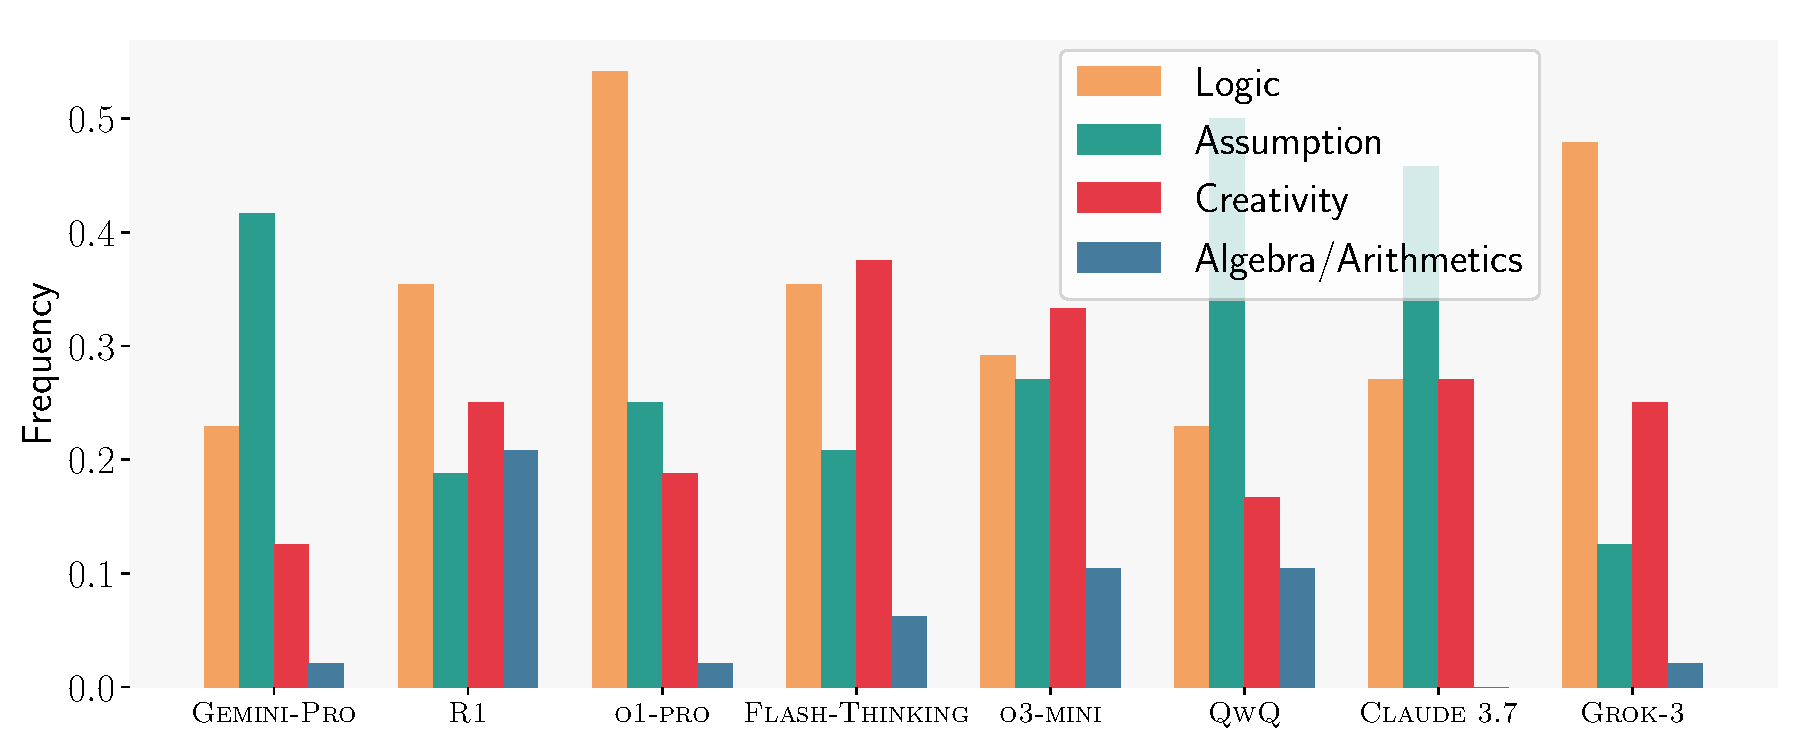
\includegraphics[width=0.9\linewidth]{figures/errors.pdf}
    \vspace{-4mm}
    \caption{Distribution of first encountered failure mode.}
    \vspace{-2mm}
    \label{fig:errors}
\end{figure}

Figure \ref{fig:errors} illustrates the distribution of these error categories as determined by our judges. The most common errors were related to flawed logic, with solutions frequently using unjustified reasoning steps, incorrect rationale, or misinterpretations of previous progress. Another significant issue was the models' tendency to treat certain critical proof steps as trivial or standard procedure without proper justification. Notably, \othree{}, despite being one of the best reasoning models, frequently skipped essential proof steps by labeling them as "trivial", even when their validity was crucial.

Another important observation is the lack of creativity in the models' reasoning. Each model often attempted the same (and wrong) solution strategy across all attempts, failing to explore alternative approaches. One exception to this observation was \flthink{}, which attempted multiple strategies in the same run, but as a consequence only shallowly explored each one, failing to reach a valid conclusion. An example of this behavior is shown in \cref{app:flthink}.


However, the models generally demonstrated strong performance in algebraic and arithmetic computations, successfully performing symbolic manipulations without external computational support. Still, \rone{} showed a notably higher frequency of algebraic or arithmetic errors, indicating a clear area for targeted improvement in this model.

\subsection{Automated Grading}\label{subsec:automated}

We explored the feasibility of replacing human graders with LLM-based evaluators, selecting \othree{} and \claude{} as grading models. Both models were provided with a grading scheme developed by our evaluators, along with a verified solution and an example evaluation for reference. In \cref{app:exp_prompt}, we provide the full prompt used for this evaluation.

As detailed in \cref{tab:llm_judge}, neither model accurately graded the solutions, consistently overestimating their quality. Specifically, the models frequently awarded points for incorrect or unjustified reasoning, inflating the scores by a factor of up to $20$.

Notably, \flthink{} and \grok{} received significantly lower scores from the automated evaluation compared to other models. We hypothesize this discrepancy arises because both tend to generate multiple solutions per attempt, or present the solutions in a chaotic manner, potentially confusing the LLM-based judges and resulting in lower scores. Conversely, \qwq{} achieved considerably higher scores, likely because it often generates simpler solution attempts, which are easier for the automated judges to interpret.

\begin{table}[t]
    \centering
    \caption{Results of automated grading executed by \othree{} and \rone{}. The table shows the average total score which is at most $42$.}
    \vspace{-1mm}
    \begin{tabular}{
        l
        x{2}{1}
        x{2}{1}
        x{2}{1}
        x{2}{1}
        }
        \toprule
        \textbf{Model} & \textbf{Ours} & {\textbf{\othree}} & {\textbf{\claude}} \\
        \midrule
        {\geminipro} & 10.1 & 19.6 & 19.3\\
        {\rone} & 2.0 & 19.3 & 14.9\\
        {\grok}& 2.0 & 15.1 & 9.1\\
        {\flthink} & 1.8 & 10.5 & 14.1\\
        {\claude} & 1.5 & 19.0 & 18.4\\
        {\qwq} & 1.2 & 23.8 & 18.8\\
        {\oone} & 1.2 & 19.3 & 21.0\\
        {\othree}& 0.9 & 19.5 & 17.1\\
        \bottomrule
    \end{tabular}
    \label{tab:llm_judge}
\end{table}